The purpose of this chapter is to provide a quantifiable assessment of the persistent radio wave energy in the near-Earth space environment due to lightning-generated whistlers. The morphology of LEP (time evolution, spatial extent at the Earth's surface, and so forth) are primarily determined by the location of wave-particle interactions; additionally, wave-particle interactions with whistlers are hypothesized to be the primary cause of slot-region electron depletions, and the ``impenetrable barrier'' below L $\sim$ 2.

Lightning-generated whistlers are sporadic, and exist alongside a multitude of radio wave activity, such as VLF chorus and plasmaspheric hiss, making a correlated \emph{in-situ} measurement challenging. Within this chapter we simulate the relative VLF energy (L-shell, latitude, longitude) in the near-Earth space environment, in volumetric units [J/$m^3$], as a means of assessing their relative contribution to the persistent radio spectrum.

%\section{Overview of Previous Work}

\section{Methodology}
Our simulation is divided into two portions: First, a simulation of persistent VLF energy due to a single flash originating at a fixed latitude, and second, an integration over a measured lightning dataset, using scaled and shifted ``stencils'' for each flash.

\section{Persistent Energy from a Single Flash}
Figure \ref{fig:power_blockdiagram} shows the steps required to compute the average energy imparted from a single lightning discharge. The resulting stencil has dimensions of L-shell and longitude.
\begin{enumerate}
\item{First we model the sub-ionosphere power spectrum generated from a flash with a known peak current, using the methodology of section \ref{section:input_power}.}
\item{We then propagate the energies through the ionosphere, using the attenuating slab approximation method of section \ref{section:trans_ionosphere_atten}.}
\item{We map the time-integrated effective power above the ionosphere (J/$m^2$ at 1000 km altitude) to an energy density along a fixed grid using a set of pre-computed ``guide rays" using the methodology in section \ref{section:raytracing}, the Landau damping from section \ref{section:damping}, and the novel interpolation scheme described below.}
\item{In order to account for multiple crossings at each grid point, and to reduce our output space across different latitudes, we store the time-averaged energy density along each field line.}
 \end{enumerate}
\begin{figure*}
\begin{center}
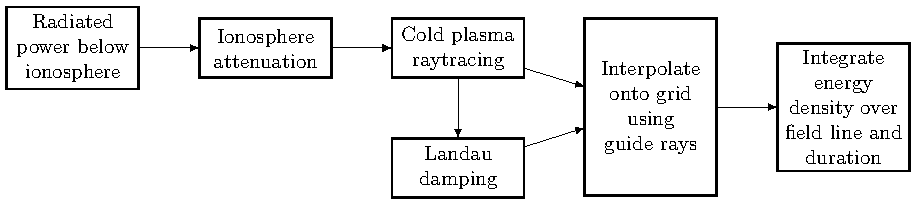
\includegraphics[width=0.8\textwidth]{figures/lightning_power_block_diagram.pdf}
\caption[Energy density calculation block diagram]{Block diagram of the average energy density calculation for a single flash.}
\label{fig:power_blockdiagram}
\end{center}
\end{figure*}


\begin{table}[h!]
\caption{Simulation Parameters}
\begin{center}

\begin{tabular}{c|c}
Ray Tracing Parameters: & \\
\hline \hline
Plasmasphere model & Simplified GCPM \\
Magnetic field model & Dipole \\
Maximum error tolerance & 1\E{-3} \\
Maximum timestep & 5 ms \\
MLT & 0 and 12 \\
K$_p$ & $\{0, 2, 4, 6, 8\}$ \\
Latitude spacing & 1$^\circ$ \\
Longitude spacing & 1$^\circ$ \\
Frequency range & 200 Hz - 30 kHz \\
Coarse Frequencies & 33 (log-spaced) \\
& \\
Grid and Interpolation Parameters: \\
\hline \hline
Fine-scale Frequencies & 50 \\
Output L-shell range & 1.2 - 8 \\
Output L-shell spacing & 0.05 \\
Output fieldline latitude spacing & 1$^\circ$ \\
\end{tabular}
%\begin{tabular}{r|c|r|c}
%ray tracing parameters: & & Interpolation parameters: & \\
%\hline
%Maximum time & 20 sec & 	Latitude spacing & 1$^\circ$ \\
%Plasmasphere model & Simplified GCPM & 	Longitude spacing & 1$^\circ$ \\
%Magnetic field model & Dipole & Frequency range & 200 Hz - 30 kHz \\
%
%%Latitude spacing & 1$^\circ$ \\
%%Longitude spacing & 1$^\circ$ \\
%%Frequency range & 200 Hz - 30 kHz \\
%%Coarse Frequencies & 33 (log-spaced) \\
%%Fine Frequencies & 50
%%
%%
%%Maximum time & 20 sec \\
%%Plasmasphere model & Simplified GCPM \\
%%Magnetic field model & Dipole 
%\end{tabular}
\end{center}
\label{tab:simulation_params}
\end{table}%

\subsection{Radiated power above the ionosphere}
Figure \ref{fig:illumination} shows the illumination below the ionosphere resulting from a single 100 kA discharge, as a function of frequency and radial distance. The illumination pattern given in equation \eqref{eqn:farfield_power_fd} is independent of location along the Earth's surface. We multiply this illumination pattern by the absorption model in section \ref{section:trans_ionosphere_atten} to determine illumination above the ionosphere. Figure \ref{fig:illumination} shows example illumination patterns for a set of flash latitudes and MLT.

% Illumination pattern
\begin{figure}[h!]
\begin{center}
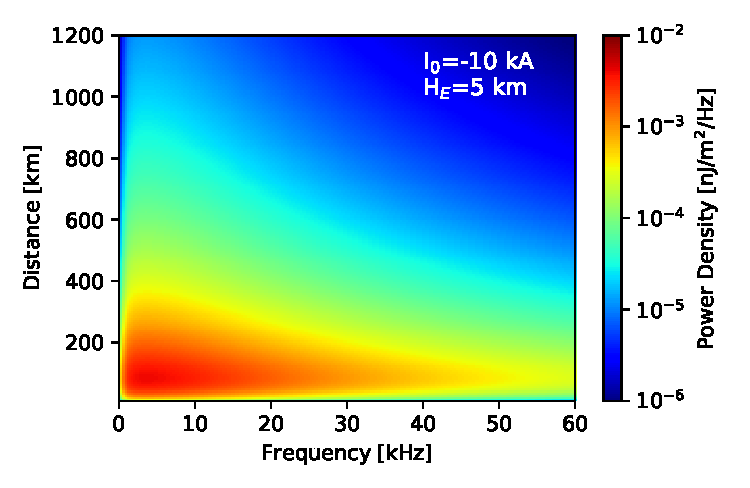
\includegraphics{figures/power_scaling_below_ionosphere.pdf}
\caption[Illumination pattern below the ionosphere]{Vertically-propagating power density below the ionosphere from a single 100kA cloud-to-ground discharge with $H_E= $5 km, as a function of frequency and radial distance. Adapted from \cite{Marshall2011}.}
\label{fig:illumination}
\end{center}
\end{figure}
% Illumination pattern
\begin{figure}[h!]
\begin{center}
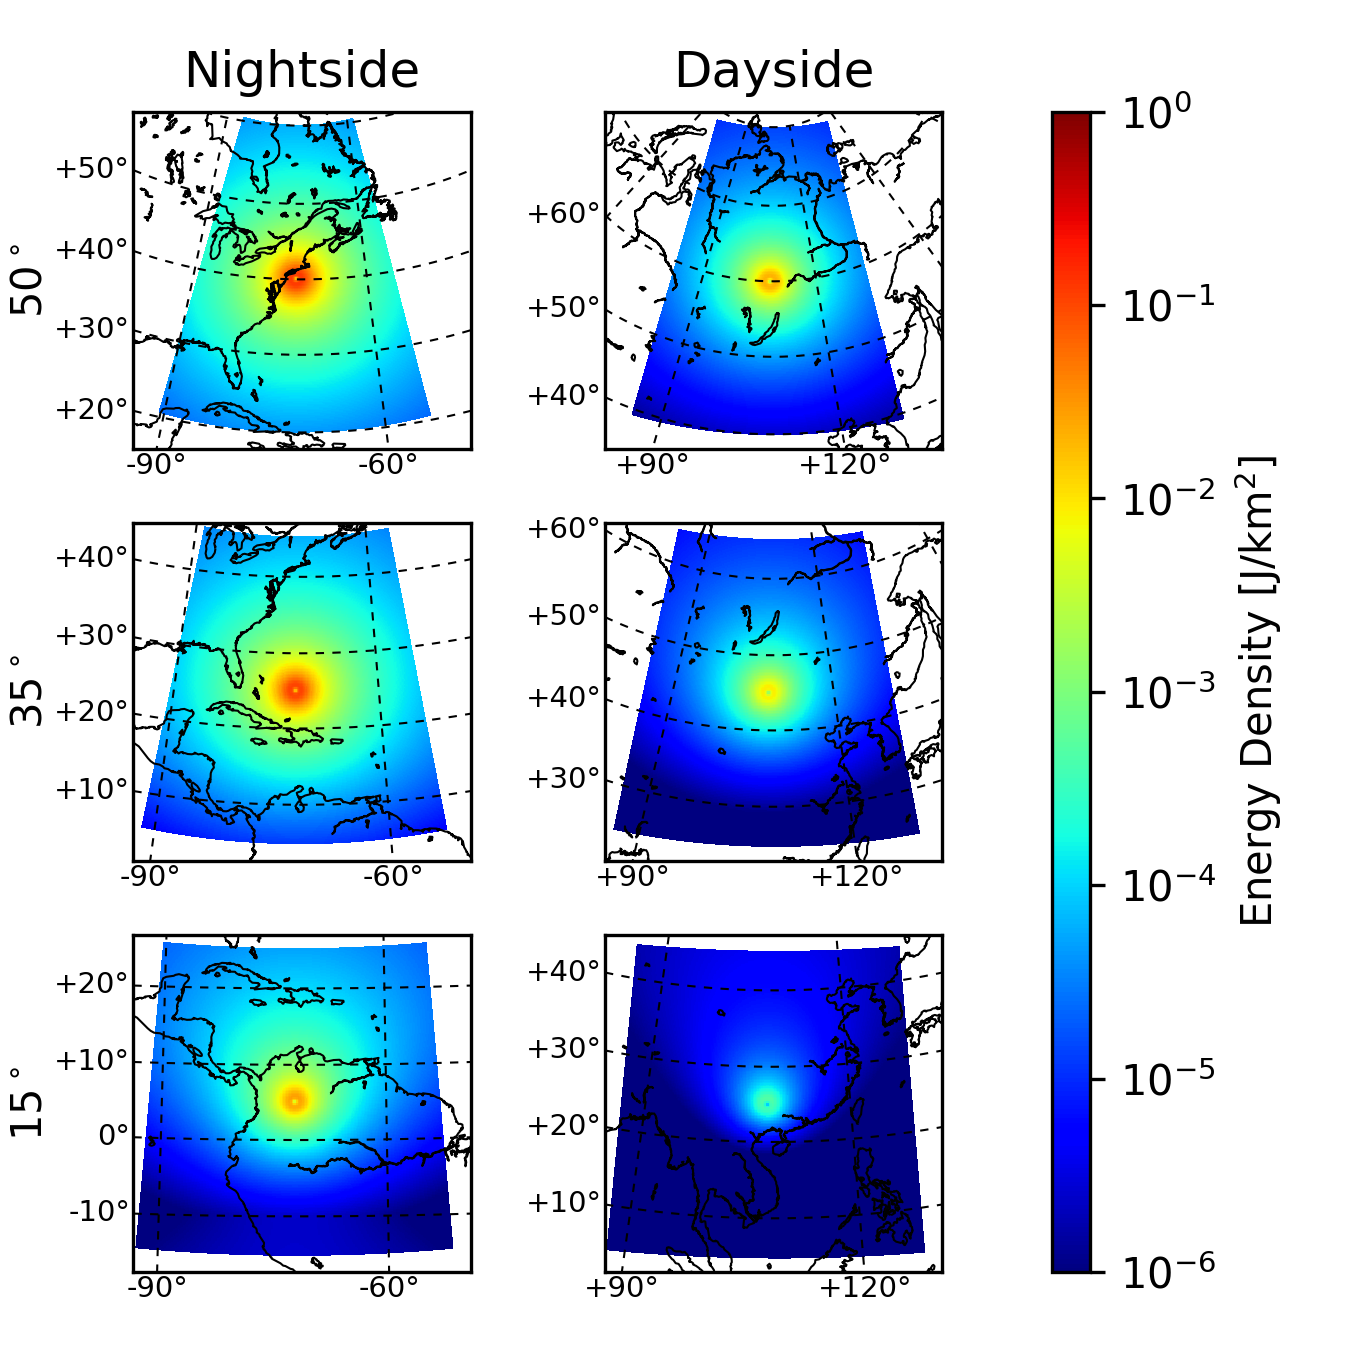
\includegraphics{figures/illumination_basemap.png}
\caption[Illumination pattern above the ionosphere]{Illumination pattern, integrated over frequency, after ionospheric attenuation (altitude = 1000 km). The ionosphere imparts stronger attenuation at equatorial latitudes, and on the dayside. The pre-ionosphere illumination pattern is toroidal, with a central null directly over the incident flash.}
\label{fig:illumination}
\end{center}
\end{figure}

By integrating over latitude, longitude, and frequency, we can estimate the total energy imparted to the magnetosphere by a flash at a given latitude, for daytime and nighttime conditions, as shown in Figure \ref{fig:illumination_totals}. Our illumination model scales with peak current squared; when combined with the updated ionosphere attenuation curves from \ref{fig:graf_curves}, we see significant overlap between day and night. A strong, midlatitude flash on the day side can easily impart similar energy as a less-intense or lower-latitude flash on the nightside.

% Total energy above ionosphere
\begin{figure}[h!]
\begin{center}
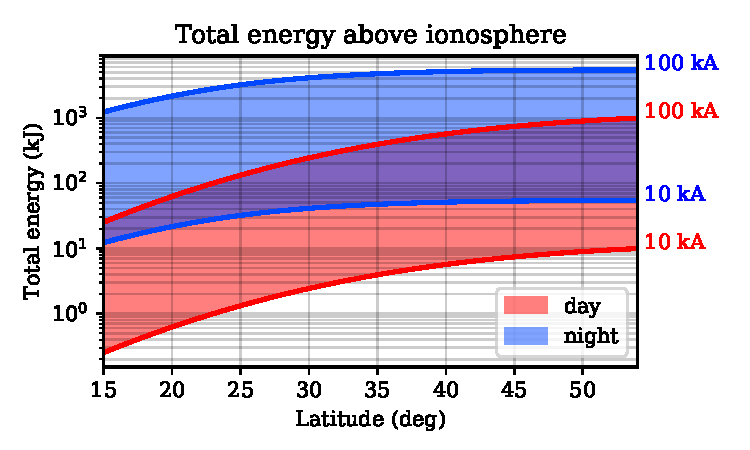
\includegraphics{figures/total_energy.pdf}
\caption[Energy above the ionosphere due to a single flash]{Integrated energy above the ionosphere from a single discharge, as a function of geomagnetic latitude. Energy scales quadratically with peak current; totals for 10 kA (an average flash), and 100 kA (a strong, but not unreasonable flash) are overlaid. The dashed lines indicate the total energy released below the ionosphere, before attenuation -- $\approx 50$ kJ for 10 kA, and $\approx 4$ MJ for 100 kA.}
\label{fig:illumination_totals}
\end{center}
\end{figure}


\subsection{Gridding and Interpolation}

We now have a model of the total energy above the ionosphere, at an altitude of 1000 km, divided into gridded bins in latitude, longitude, and frequency. The next step required is to map the energy within each cell out into the plasmasphere. We accomplish this task using a ``guide ray'' formulation, as illustrated in Figure \ref{fig:interpolation_scheme}.

Using the ray tracing and Landau damping technique from section \ref{section:raytracing}, we compute rays in 1$^\circ$ steps in both latitude and longitude, within 1000 km of the incident flash, for 33 logarithmically-spaced frequencies between 200 Hz and 30 kHz. Rays are computed for 20 seconds. See table \ref{tab:simulation_params} for a list of various parameters used. In order to generalize across all longitudes, we use the dipole magnetic field model and the simplified GCPM plasmasphere model. Additionally, we restrict raytracing deviation to the meridional plane to omit any numerical instabilities introduced. The computed rays are then interpolated onto a uniform time axis using one-dimensional linear interpolation for each parameter. 

We make the assumption that the energy bounded by the set of 8 guide rays (two latitudes, two longitudes, two frequencies) remains bounded by these rays as they propagate. Furthermore, we assume that our interpolated timesteps are much larger than the envelope of the wave packet (see Figure \ref{fig:lightning_spectrum}). Therefore, the initial energy within each cell is bounded by a four-dimensional voxel, determined by two adjacent timesteps $t_{n-1}, t_n$ of the guide ray set \{(lat$_1$, lat$_2$), (lon$_1$, lon$_2$), (f$_1$, f$_2$)\}.

Next, we map the energy within each voxel to our output grid coordinates -- chosen here to be 1$^\circ$ steps in latitude, 0.25$^\circ$ in longitude, and 0.05 L-shell. We accomplish this task using an n-dimensional Delaunay triangulation construction \citep{Delaunay1934, Lee1980}. A Delaunay triangulation breaks the convex hull of a volume, as defined by a set of points in $\mathbb R^n$, into a set of primitive shapes called ``simplexes''. Each simplex is an n-dimensional triangle. 

At each timestep, we compute a Delaunay triangulation for the 16 points defined by corners at \{($t_{n-1}, t_n$), (lat$_1$, lat$_2$), (lon$_1$, lon$_2$), (f$_1$, f$_2$)\}. Once a Delaunay triangulation has been made, it is a computationally-efficient task to check whether or not an arbitrary new point is within any of the simplexes. We use the Scipy Delaunay implementation, which is based on the open-source \emph{qhull} code \citep{Barber1996}. For any point within the volume, we assign to it the average energy density in $J/m^3$ within the voxel at the given timestep, multiplied by the average Landau damping factor. Figure \ref{fig:delaunay_1} illustrates the interpolation method.

\subsubsection{Fine-scale frequency interpolation}
Our output grid coordinates are given in three dimensions -- latitude, longitude, and L-shell. However, our Delaunay construction adds an additional dimension, frequency. We can perform a fine-scale interpolation on the frequency axis by selecting a linearly-spaced grid of sub-frequencies between the two ray frequencies $f_1, f_2$. Checking and logging whether or not each new point is within the four-dimensional voxel is equivalent to interpolating and checking in three dimensions, as illustrated in Figure \ref{fig:delaunay_2}.

    \begin{figure}[h!]
    \centering
    \begin{subfigure}[t]{0.45\textwidth}
    \centering
        	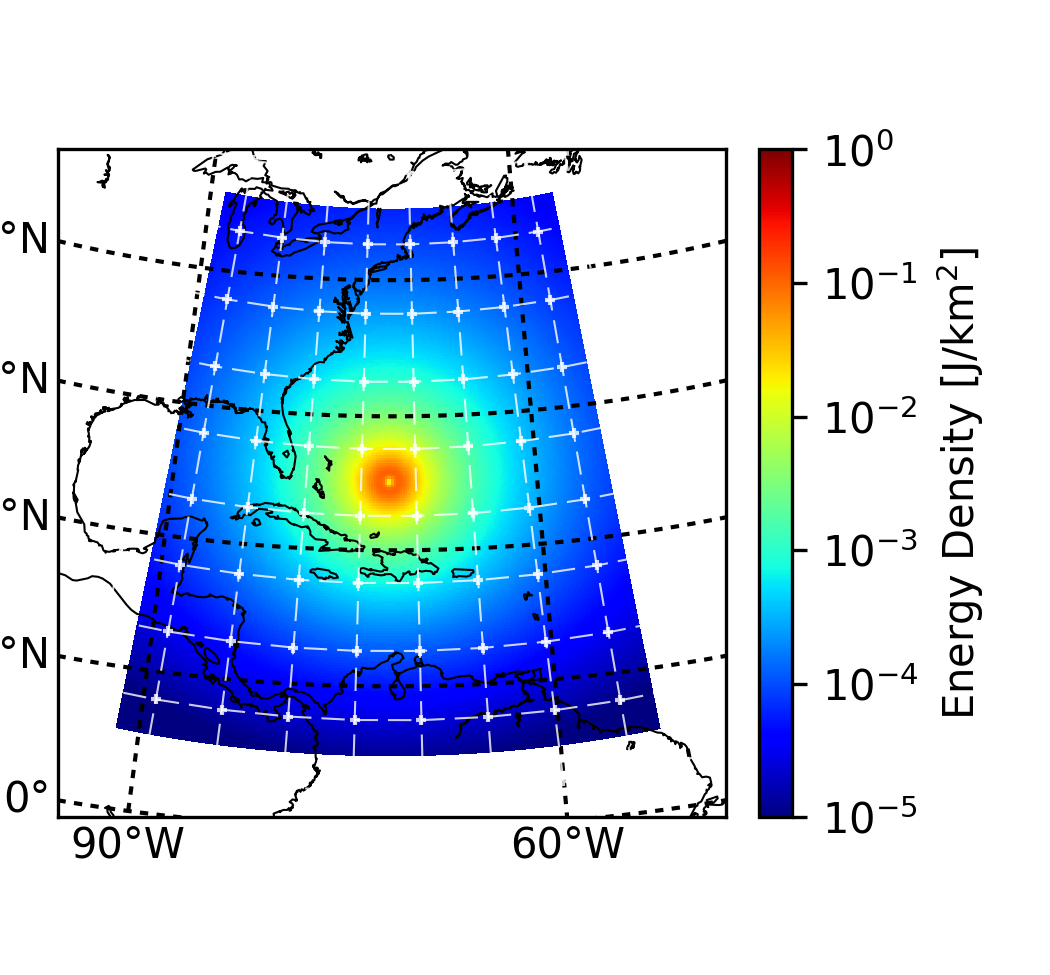
\includegraphics{figures/input_energy_with_grid.png}
	\caption{Input energy gridding}
        \label{fig:input_energy_grid}
    \end{subfigure}\hfill
    \begin{subfigure}[t]{0.45\textwidth}
    \centering
        	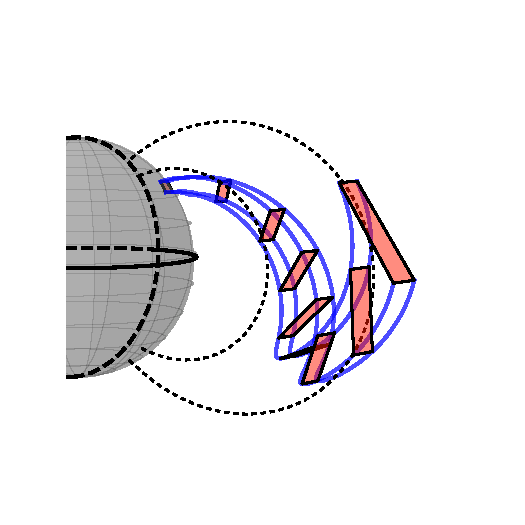
\includegraphics[trim={1cm 0.25cm 1cm 1cm},clip]{figures/interpolation_globe1.pdf}
	\caption{``guide ray'' construction}
        \label{fig:guide_rays}
    \end{subfigure}
    \caption[Illustrations of the interpolation scheme]{An illustration of the interpolation scheme. (a) Energy at the top of the ionosphere is divided into cells, in latitude, longitude, and frequency. Shown here with 5$^\circ$ cells (much larger than used in simulation). The plotted energy is integrated over frequency. (b) Illustration of the guide ray method. Input energy is integrated between a set of guide rays, spaced in latitude, longitude, and frequency. This energy is then averaged over a 4-dimensional volume, bounded by two adjacent timesteps $t_{n-1}$, $t_n$ of the guide rays.}
    \label{fig:interpolation_scheme}
\end{figure}


% Delaunay figure
\begin{figure}[h!]
\begin{center}
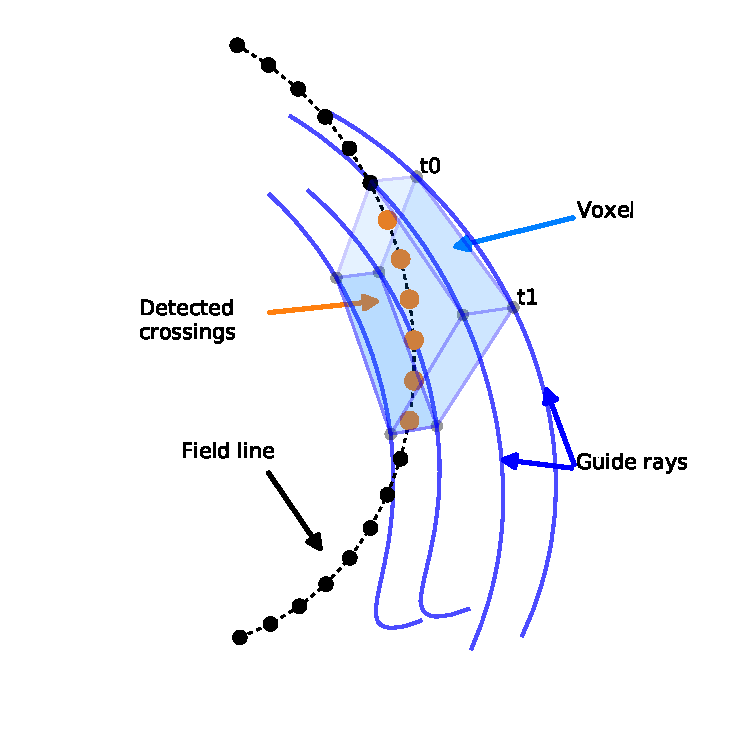
\includegraphics{figures/delaunay_1.pdf}
\caption[Delaunay interpolation method]{Illustration of the Delaunay interpolation method, shown here in three dimensions (e.g., for a single frequency).}
\label{fig:delaunay_1}
\end{center}
\end{figure}

% Fine-scale frequency interpolation
\begin{figure}[h!]
\begin{center}
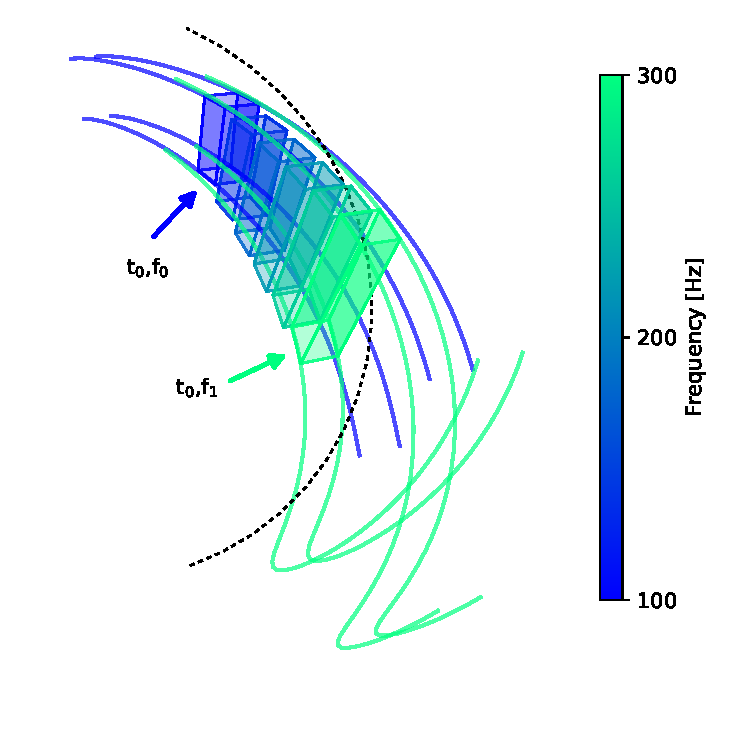
\includegraphics{figures/delaunay_2.pdf}
\caption[Fine-scale frequency interpolation]{An illustration of fine-scale frequency interpolation. Here we show a three-dimensional voxel being linearly interpolated between two sets of guide rays, at $f_1=200$ Hz and $f_2=300$ Hz. Our implementation operates on a four-dimensional voxel, facilitating rapid checking across fine-scale frequency interpolation steps.}
\label{fig:delaunay_2}
\end{center}
\end{figure}

\subsubsection{Discussion}
Our interpolation method differs substantially from \cite{Bortnik2005} and related work. \citeauthor{Bortnik2005} performed an area-weighted interpolation between guide rays in latitude and frequency, and then looked for ray-segment intersections with cross-sectional areas perpendicular to a field line. Crossings, however, are exceedingly rare over the full set of guide rays and output cross-sectional area segments, which requires clever restriction of the output space, or high computational resources. Our method was selected for computational efficiency when relaxing the meridional-plane restriction, and to assure that all input energy is accounted for. Using the \cite{Bortnik2005} method with larger intervals in latitude and longitude can result in undersampling the post-ionosphere illumination pattern, while our method integrates the input energy regardless of grid size.

One caveat of our interpolation algorithm is that the Delaunay triangulation implementation only checks whether or not a point is within the convex hull of the voxel, rather than the voxel itself. For simple voxels, and at early timesteps (e.g., before any magnetospheric reflection), we can be confident that the voxel remains cubic, and the concave and convex hulls are equivalent. However at later timesteps, after the rays have spread and reflected substantially, the concave and convex hulls are likely not equivalent, in which case the interpolation algorithm may artificially disperse the energy over a larger volume, effectively underestimating energy density while overestimating energy spreading. Figure \ref{fig:convex_hulls} shows some simple polygons and their convex hulls.
% CONVEX HULL FIGURE
\begin{figure}[h]
\begin{center}
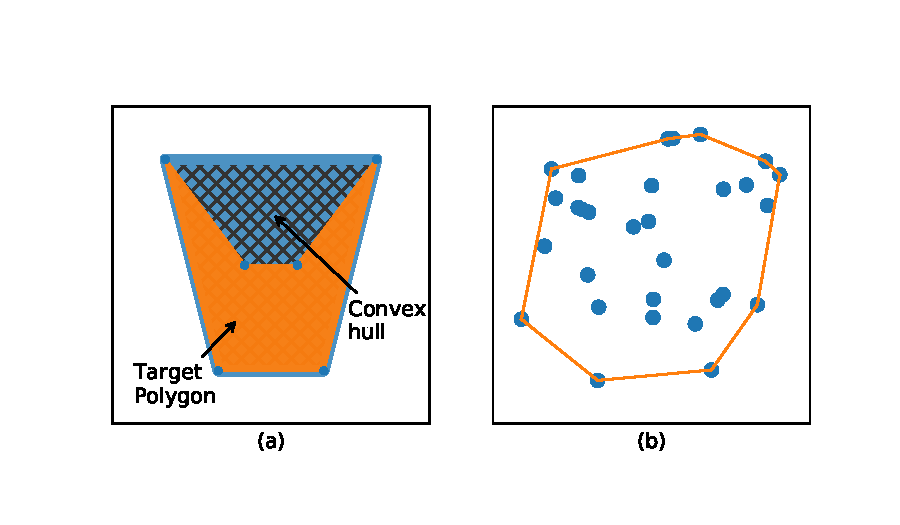
\includegraphics{figures/convex_hulls.pdf}
\caption[Qualitative illustration of convex and concave hulls]{Illustration of a convex hull in two dimensions. (a) A simple polygon, shown in orange, for which the convex hull and concave hulls differ substantially. (b) A collection of random points, and their concave hull.}
\label{fig:convex_hulls}
\end{center}
\end{figure}


\subsection{Energy imparted by a single flash}
The assembled model of a single flash is parameterized by a flash location (latitude, MLT), and K$_p$; the output space can be specified over time, latitude, longitude, L-shell, and frequency. We can reduce the parameter space by integrating over various axes.

Figure \ref{fig:energy_from_single_flash} shows the energy density in the meridional plane, integrated over time and frequency, and averaged over a 0.25$^\circ$ slab in longitude (Note that wave intensity is strongest with a slight offset ($\sim 100$ km) in longitude -- see section \ref{section:longitude_scaling}). Energy launched from lower latitudes remains bounded in latitude as it propagates outward; conversely, higher-latitude flashes exhibit more spread in latitude along a fieldline. Higher-latitude flashes also exhibit a stronger ``duct-like'' enhancement in which energy is well-guided along a fieldline, which we can attribute to the more-gradual curvature of the field line before the first magnetospheric reflection. Lower-latitude flashes encounter stronger field line curvature, and therefore begin to disperse earlier. 

Figure \ref{fig:wave_energy_timeseries} shows similar data, now volume-averaged over each fieldline, to show the time evolution. In all cases, the most-intense and most-coherent portion of the wave packet disperses within the first $\sim$ 3 seconds. Again, lower-latitude flashes exhibit greater spread in L-shell. Increasing K$_p$, which brings the plasmapause closer to the Earth, constrains energy within the plasmasphere, both by reflection from the sharp density gradient, and by increased Landau attenuation due to the increased temperature outside the plasmapause from the thermal model in section \ref{section:damping}. However the closer plasmapause has little effect until at least K$_p \sim 4$; for K$_p$ values less than 4, the plasmapause remains well above the normal extent of wave energy. 

\begin{figure}[h!]
\begin{center}
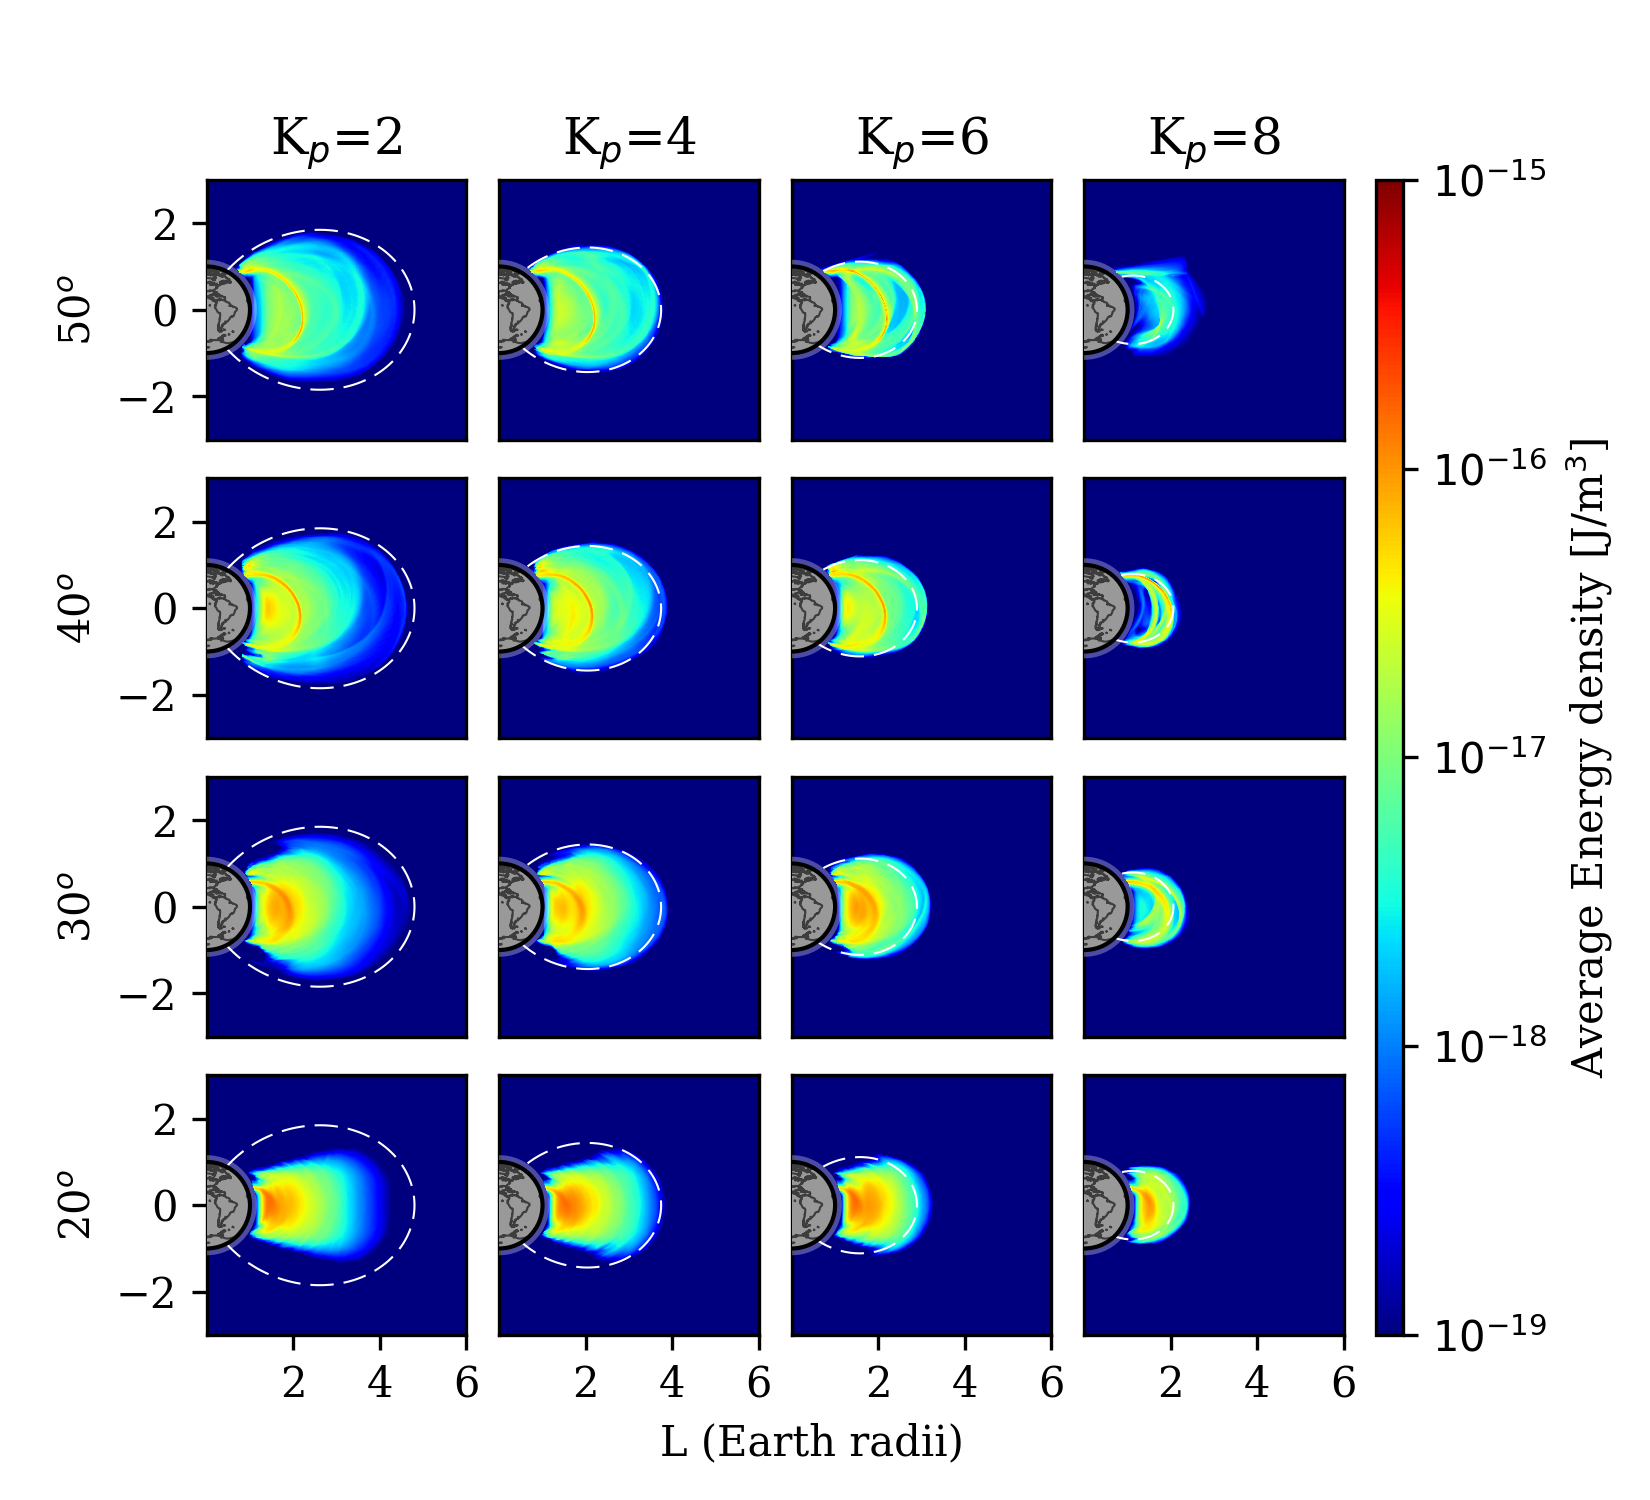
\includegraphics{figures/energy_from_single_flash_meridonal_plane.png}
\caption[Energy density in the meridional plane for a single flash]{Meridional-plane energy densities for a single flash, shown for a variety of input flash latitudes and geomagnetic conditions.}
\label{fig:energy_from_single_flash}
\end{center}
\end{figure}

\begin{figure}
\begin{center}
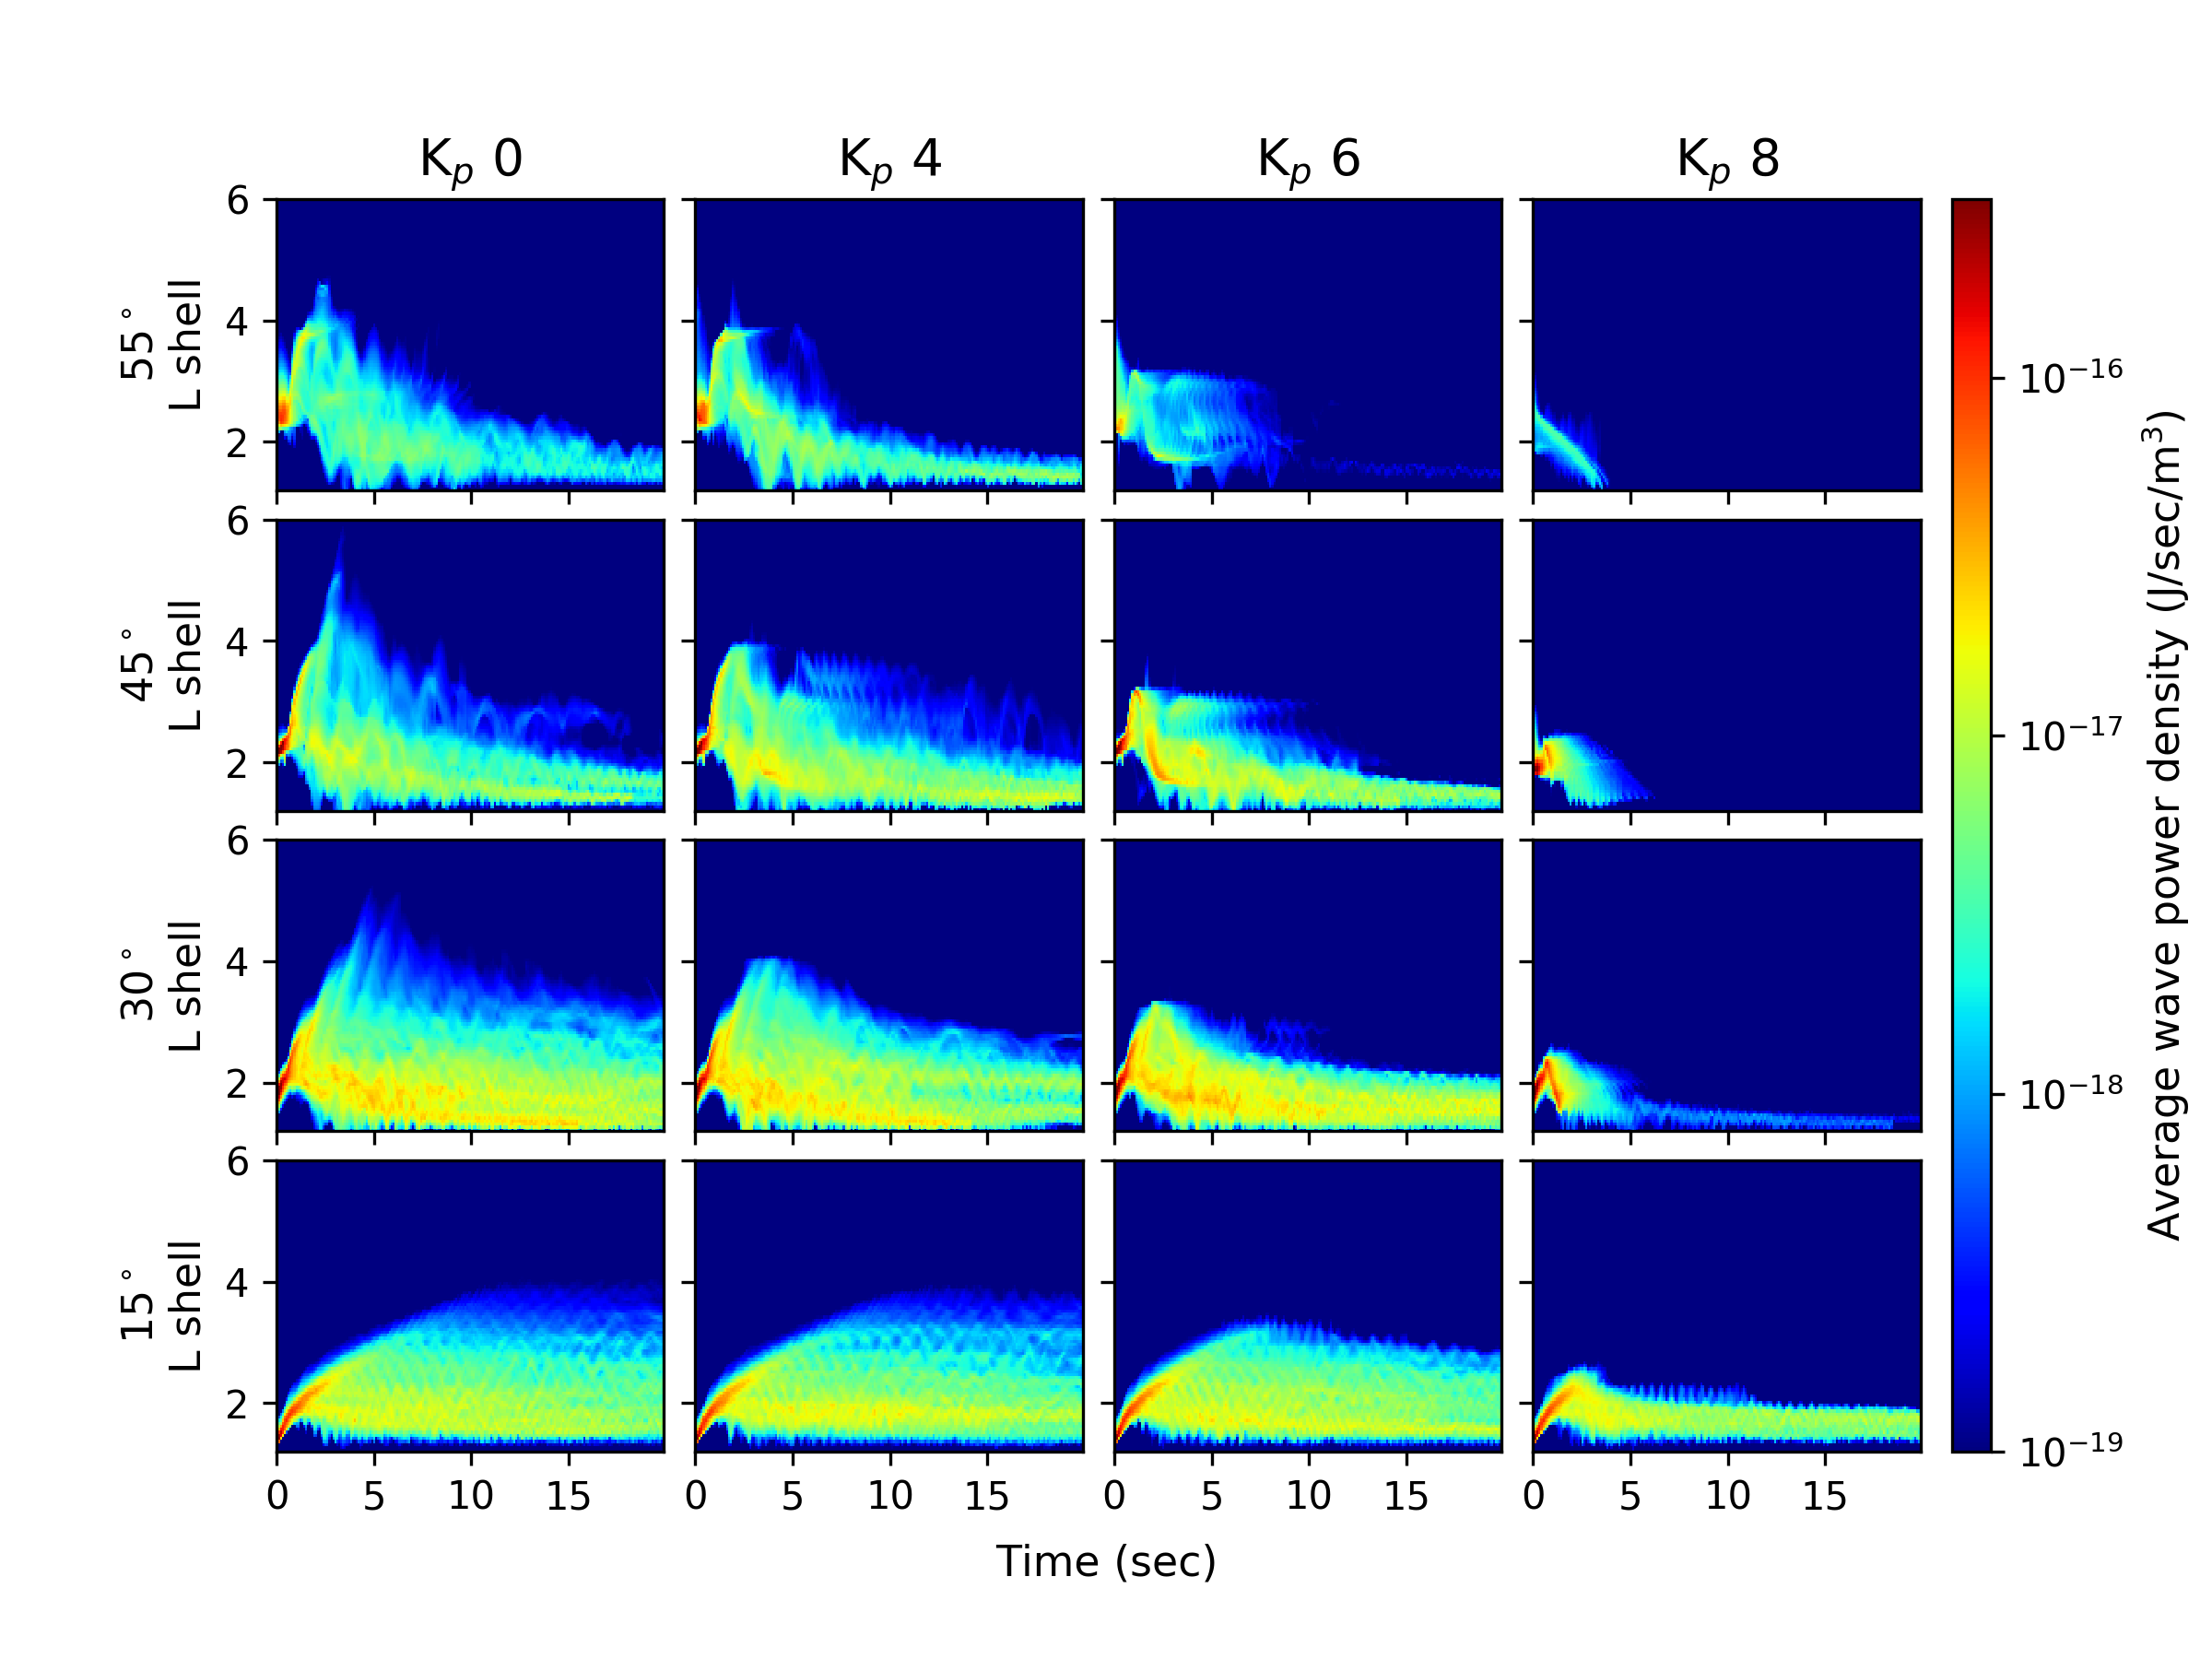
\includegraphics[angle=-90]{figures/wave_energy_timeseries_vs_L.png}
\caption[Energy density vs time vs L-shell]{Energy density time series plots, for a range of flash latitudes and geomagnetic conditions. Energy is averaged over a 0.25$^\circ$ section in longitude, centered over the flash.}
\label{fig:wave_energy_timeseries}
\end{center}
\end{figure}

\section{Global Energy Density}
In order to estimate the global persistent VLF energy density within the magnetosphere, we first precompute the average energy imparted by a flash at an array of latitudes, for the dayside and nightside, which form our stencil array. We note that our illumination model scales with peak current squared ($E \propto I_0^2$), and that the propagation process is assumed to be linear -- that is, spatially-coincident flashes have no cumulative effect on each other. We can then simply shift and scale our stencils according to lightning measured from GLD360, and sum / average the result. 

Stencils are computed for 1$^\circ$ steps, ranging between 15$^\circ$ and 55$^\circ$ in geomagnetic latitude. Noting that the plasmasphere density model is symmetric north / south, and that the magnetic field model is symmetric with the exception of polarity, we assume the impact of a southern hemisphere flash is identical to that of a field-line-coincident northern hemisphere flash. Longitude variation is computed in 0.25$^\circ$ steps, with a maximum extent of 20$^\circ$ from the flash location. We compute stencils for two MLT values, 0 and 12, representing the nightside and dayside, and select a stencil set accordingly for each flash. Finally, we compute stencils for an array of K$_p$ values -- \{0, 2, 4, 6, 8\} -- and linearly interpolate along this axis for measured values of K$_p$.

Figure \ref{fig:energy_stencils} shows a grid of nightside energy stencils for several latitudes and several K$_p$.

\begin{figure}[h!]
\begin{center}
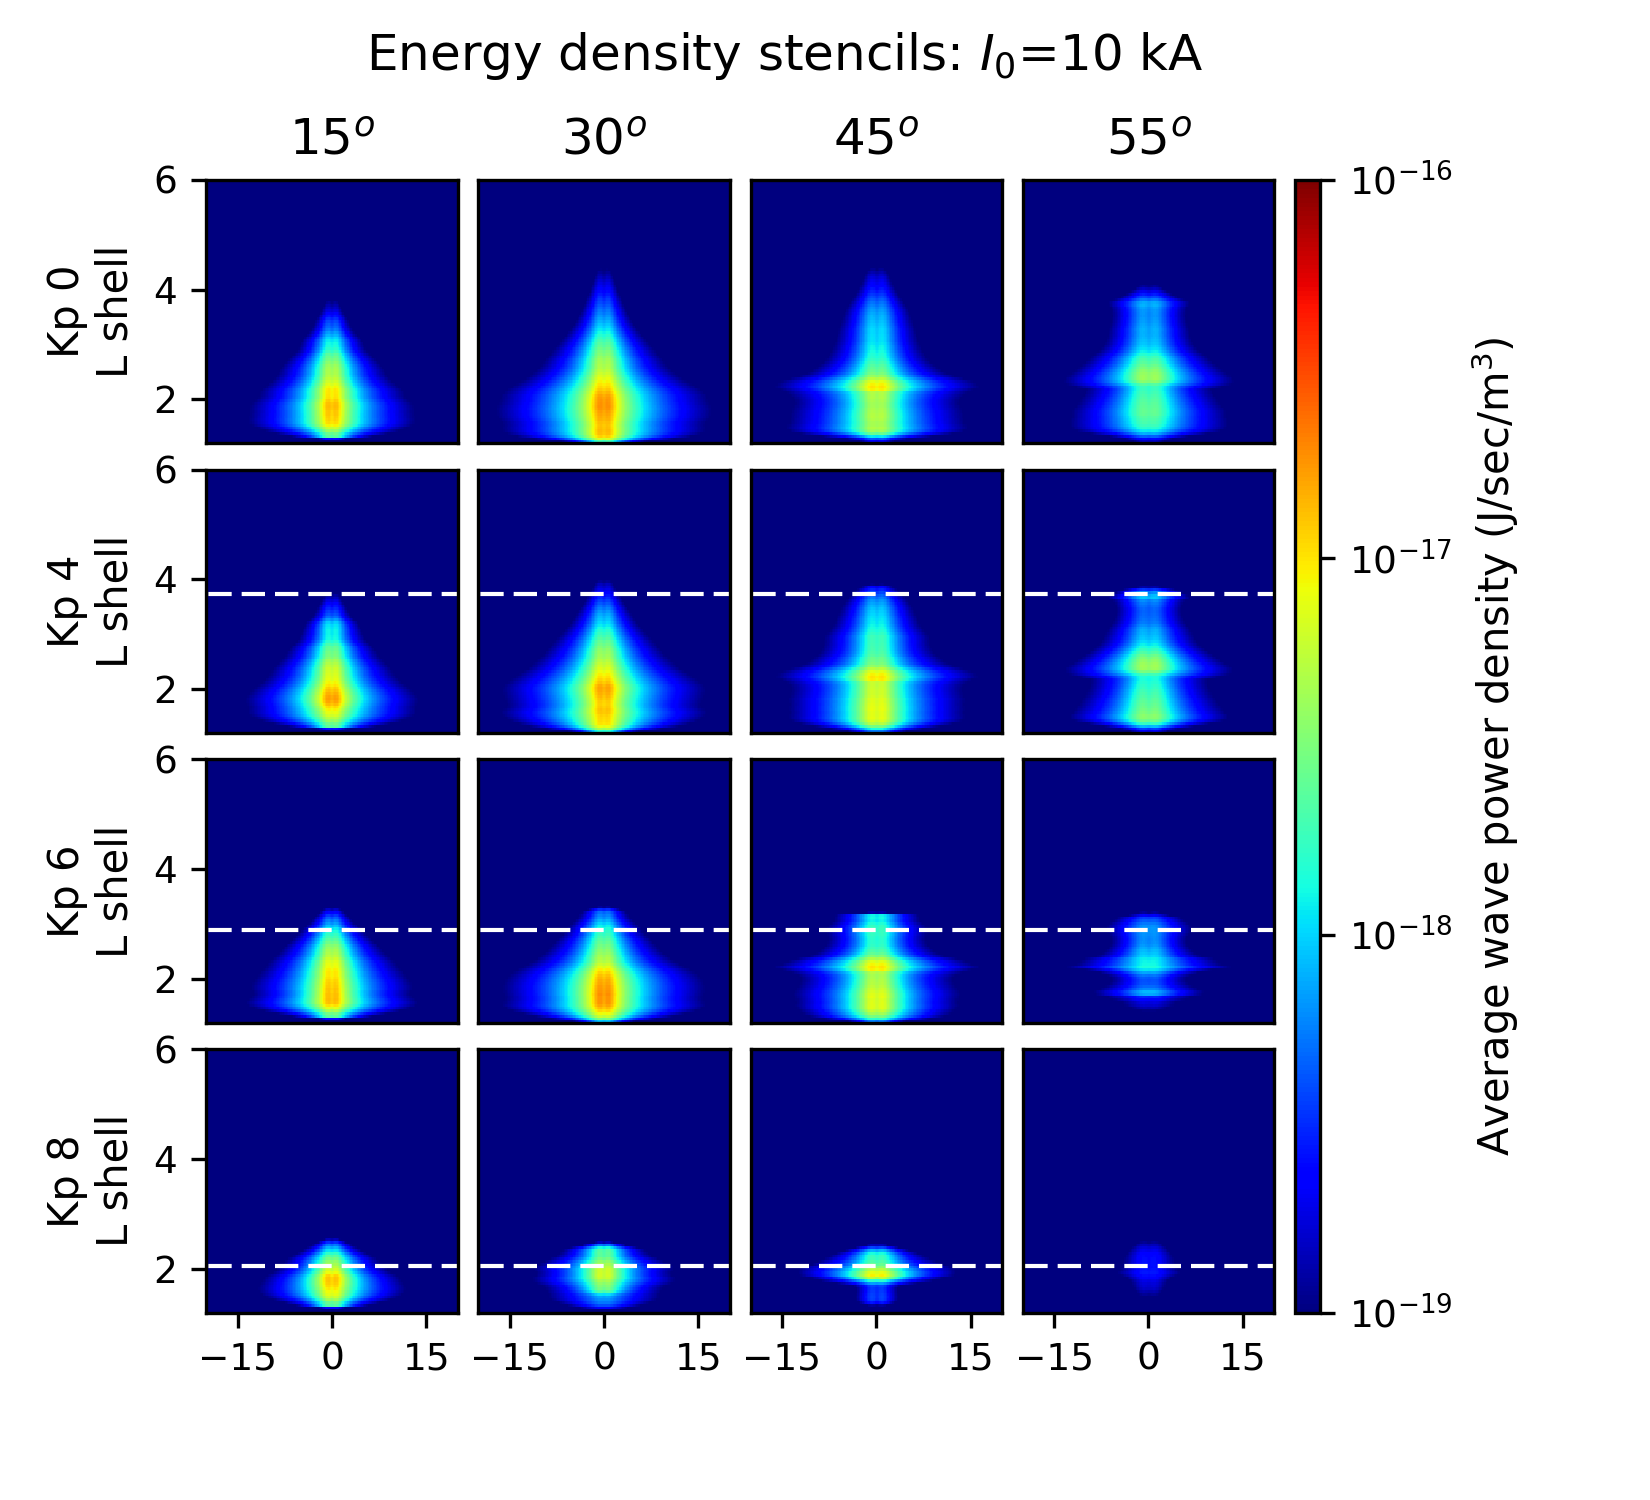
\includegraphics{figures/wave_energy_vs_L_stencils.png}
\caption[Energy density stencils]{Energy density stencils for a range of flash latitudes and geomagnetic conditions, for a nightside, 10 kA flash. The dashed white lines indicate the location of the plasmapause, which is brought closer to the Earth with increasing $K_p$.}
\label{fig:energy_stencils}
\end{center}
\end{figure}

\section{Longitude Dependence}
\label{section:longitude_scaling}
As mentioned previously, our ray tracing is confined to the meridional plane axis, with no deviation along the longitudinal axis. In order to greatly reduce computation time and storage requirements, it is desirable to find a scaling function with respect to longitude, so that we need only compute power densities along a single meridional plane slice (e.g., a fixed longitude, offset from the initial flash), and simply weight it accordingly to compute a full 3D solution. \cite{Lauben1998} chose a longitude scaling function according to the assumed peak resonance frequency; similarly, \cite{Bortnik2005}, noting that the model is entirely linear, chose a longitude scaling function to be the ratio of input powers from equation \eqref{eqn:farfield_power_fd}

\begin{eqnarray}
F(\phi) & = & \frac{S(\phi)}{S(\phi_0)} \\
& = & \frac{\sin^2\theta/r^2}{\sin^2\theta_0/r_0^2}
\label{eqn:bortnik_longitude_scaling}
\end{eqnarray}
\noindent where $\phi$ and $\phi_0$ are the offset and reference longitudes, $\theta$ and $\theta_0$ are the zenith angles, and $r$ and $r_0$ are the radial distance from the input flash. Note that the frequency dependence terms cancel out nicely, as there is no change in the frequency terms with respect to longitude. In order to avoid the central null directly above the incident flash, \citeauthor{Bortnik2005} uses a longitude offset of $\sim 1^\circ$ for the reference slice.

The power-ratio scaling factor is completely accurate, so long as we consider only rays launched from the same latitude as the incident flash. However, scaling our model \emph{output} according to model \emph{input} is somewhat of a compromise, as the total meridional-plane power is the result of a scaled family of rays, launched from a range of latitudes. Each latitude has a slightly different longitude offset, and will in actuality be further from the flash than the power scaling in equation \eqref{eqn:bortnik_longitude_scaling} predicts; the net result will be a slight overestimation of power along the scaled longitudinal axis. Furthermore, the effect is more-prominent closer to the incident flash, where input energies are strongest. 

Figure \ref{fig:longitude_scaling_diagram} illustrates the scaling geometry. The dashed black lines show the meridional plane slices above the flash, at the reference longitude, and at the target longitude to be scaled. Blue lines indicate the true distance from the flash, and the red line indicates the distance used in the 2D scaling. Contour lines denote radial distance from the flash, in kilometers. 

Using the full 3D solution, we can examine whether or not a single scaling function will work for all latitudes within a given stencil. Figure \ref{fig:longitude_scaling_per_latitude} shows the normalized scaling factor as a function of longitude offset from the incident flash, for each latitude in the stencil, for 5$^\circ$ increments in flash latitude. Lower-latitude flashes exhibit a wider spread in scaling; the spread reduces as the flash latitude increases, reaching a minimum at $\sim$ 35$^\circ$, and broadening out again at higher latitudes.

\begin{figure}[h!]
\begin{center}
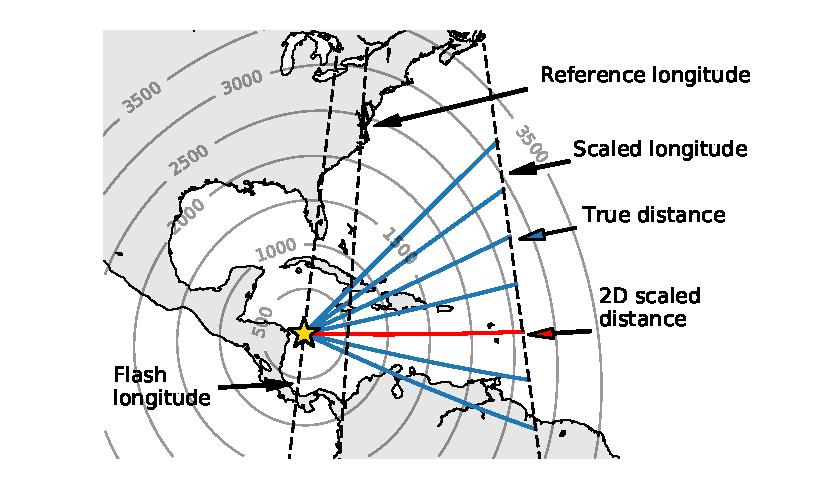
\includegraphics{figures/longitude_scaling_diagram.pdf}
\caption[2D vs 3D longitude scaling geometries]{Illustration of the geometries involved in scaling along the longitudinal axis.}
\label{fig:longitude_scaling_diagram}
\end{center}
\end{figure}

\begin{figure}[h!]
\begin{center}
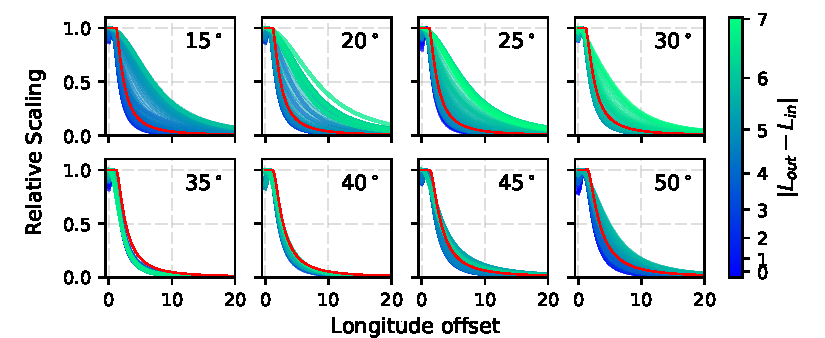
\includegraphics{figures/longitude_scaling_per_latitude_with_colorbar.pdf}
\caption[Relative longitude scaling factors per latitude]{Plots of the relative longitude scaling factors for a set of flashes, between 15$^\circ$ and 50$^\circ$, in 5-degree increments. Each line is normalized by its value at the reference longitude, for a given latitude offset from the flash. The spread in scaling factors is broad at lower-latitude flashes, becoming more-consistent at mid-latitudes, and broadening out again at high latitudes. Red lines indicate the 2D scaling function in equation \eqref{eqn:bortnik_longitude_scaling}).}
\label{fig:longitude_scaling_per_latitude}
\end{center}
\end{figure}

Our 3D implementation computes the meridional-plane power density along each offset longitude, using true scaling for each set of guide rays. Figure \ref{fig:longitude_scaling_2d_vs_3d} compares our full 3D weighting with the \cite{Bortnik2005} scaling method. For longitudes less than the reference longitude, we use the reference longitude result, in order to compensate for the central null. Signed, relative errors are shown with respect to the mean of both models, which produces a sigmoid function with asymptotes at $\pm$ 200\%:
\begin{equation}
\epsilon = \frac{P_{2D} - P_{3D}}{(P_{2D} + P_{3D})/2}
\end{equation}

Figure \ref{fig:longitude_scaling_total} shows the average error across the entire stencil versus K$_p$ and longitude.At lower latitudes, the 2D scaling method overestimates power by $\sim$ 5\%; however at higher latitudes the 2D method can overestimate energy density by 20 \% or more.
\begin{figure}[h!]
\begin{center}
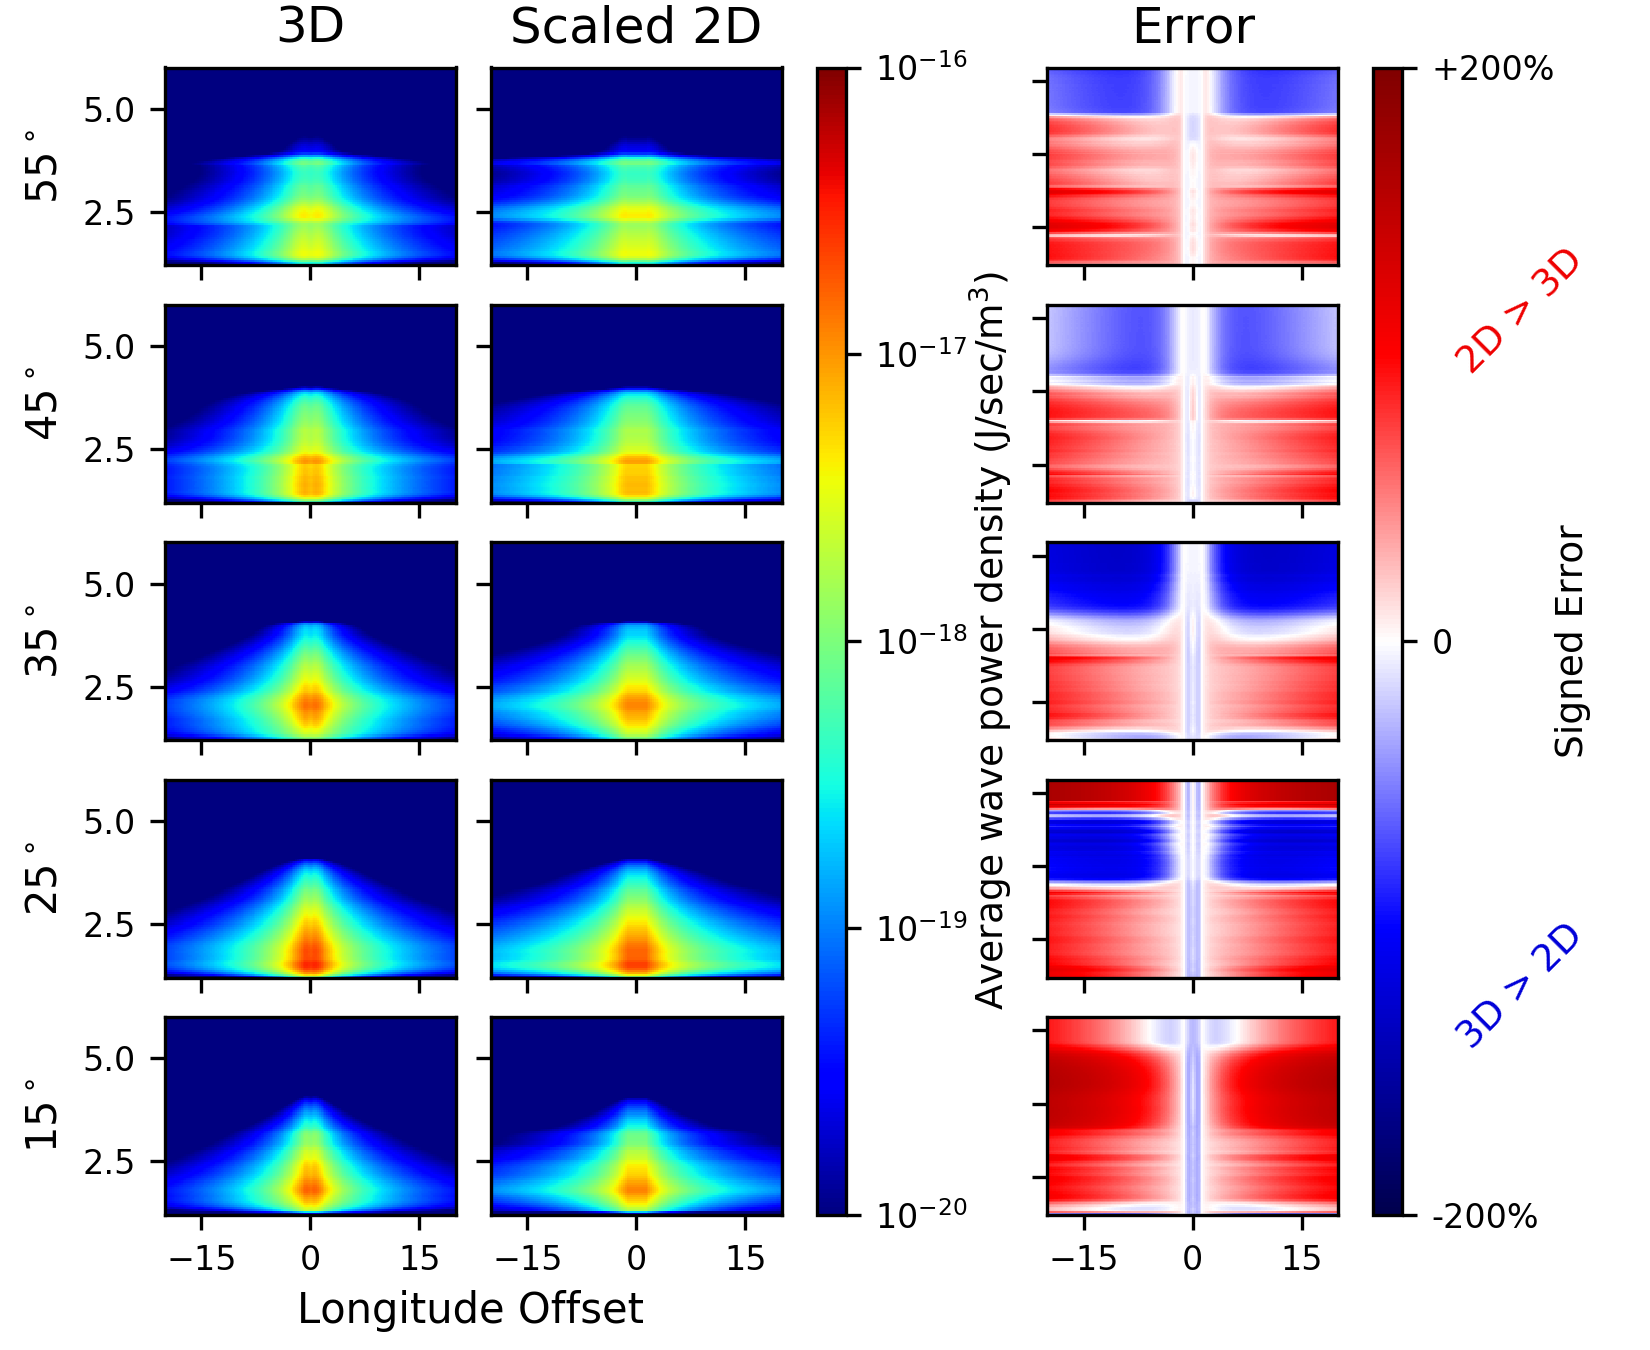
\includegraphics{figures/rel_error_grid_2d3d.png}
\caption[Difference between 2d and 3d longitude scaling]{A comparison of meridonal-plane power density stencils, using the full 3D solution and the scaled 2D solution, for K$_p$ = 4. The rightmost column shows the signed relative error on a per-pixel basis.}
\label{fig:longitude_scaling_2d_vs_3d}
\end{center}
\end{figure}

\begin{figure}[h!]
\begin{center}
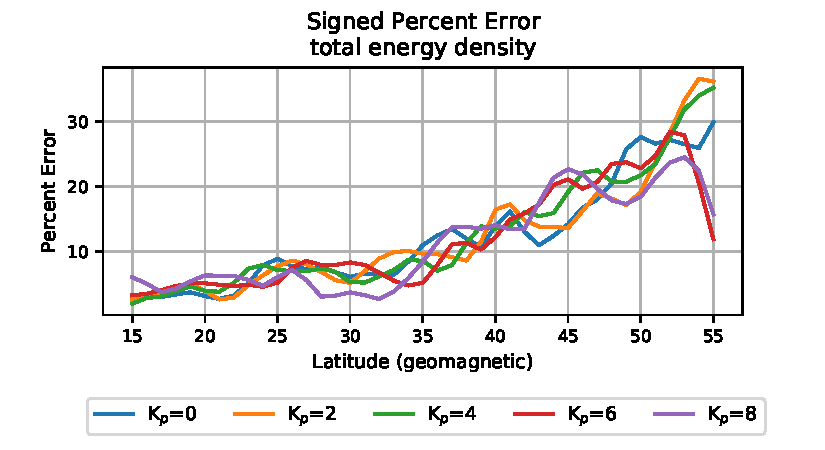
\includegraphics{figures/longitude_scaling_total_error.pdf}
\caption[Total percent error in 2D scaling]{Total signed percentage error between stencils generated with the 2D scaling technique and the full 3D scaling method. On average, the longitude scaling function in equation \eqref{eqn:bortnik_longitude_scaling} overestimates energy density by $\sim 15\%$.}
\label{fig:longitude_scaling_total}
\end{center}
\end{figure}

\subsection{Results of the global model}
We apply the shifted and scaled stencil technique to the GLD360 dataset, for all detected flashes between August 2014 and April 2016. Flashes are then binned into dayside and nightside by quantizing magnetic local time:

\begin{eqnarray}
\label{eqn:MLT}
MLT & = & \mathrm{UT} + (\phi_{\rm{flash}} - \phi_{\rm{ut}})/15 \\
\mathrm{Day} & \equiv & 6 < MLT \leq 18 \\
\mathrm{Night} & \equiv & (MLT \leq 6) \parallel (MLT > 18)
\end{eqnarray}
\noindent where $\phi_{flash}$ is the magnetic longitude of the incident flash, UT is the fractional hour of day in universal time, and $\phi_{ut}$ is the UT reference magnetic longitude of Greenwich \citep{Laundal2016}.

We use historical K$_p$ values corresponding to each flash. However we replace K$_p$ with K$_{p(max)}$, as in \cite{Carpenter1992}, in order to better align with the plasmasphere model used. K$_{p(max)}$ is defined as the maximum value of K$_p$ within the preceding 24-hour period.

\begin{figure}[ht!]
\begin{center}
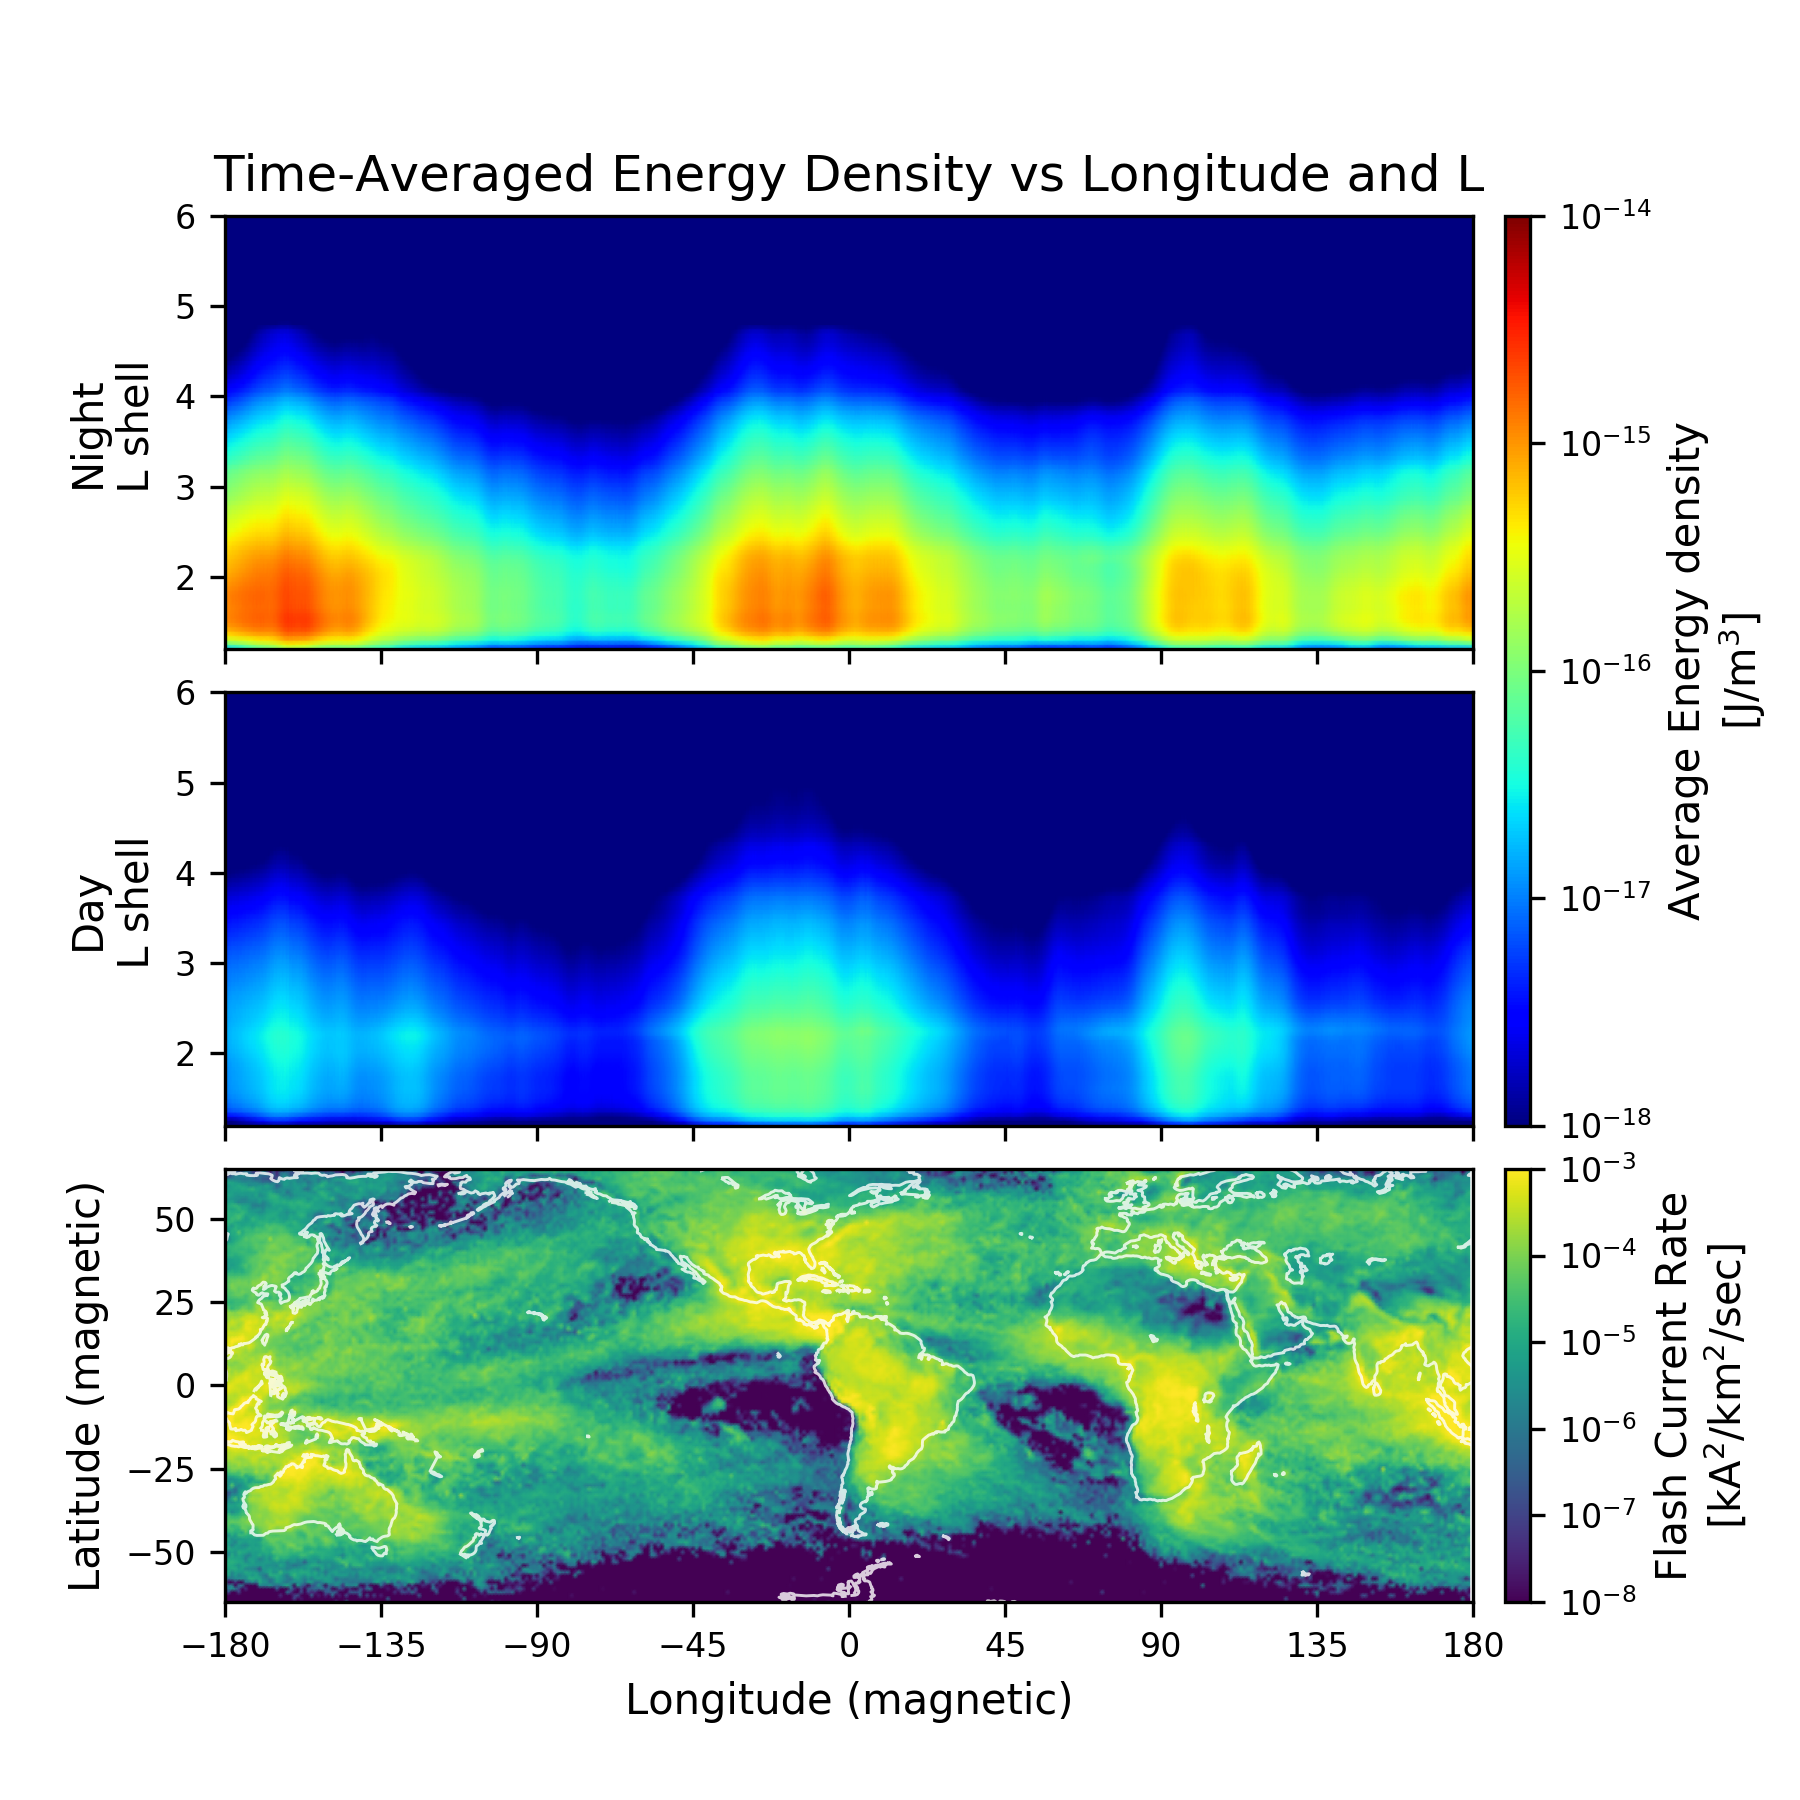
\includegraphics{figures/Energy_density_daynite.png}
\caption[Average energy density vs longitude and L]{Average energy density as a function of L-shell and geomagnetic longitude. The top plot shows the nightside only, and the middle plot shows dayside only. The bottom plot shows the corresponding peak current distribution input into the model.}
\label{fig:energy_density_daynite}
\end{center}
\end{figure}

Figure \ref{fig:energy_density_daynite} shows the resulting energy density, averaged over the entire date range, broken out into day and night. Figures \ref{fig:energy_density_vs_L_trendline} and \ref{fig:energy_density_vs_L_multiple_kp} show the results averaged across the all longitudes.

As shown in Figure \ref{fig:energy_density_vs_L_trendline}, energy density falls off logarithmically with respect to L. The cumulative effect of the plasmapause, the variance of which is taken into effect via multiple K$_p$ values, results in an additional dropoff at L $\sim$ 4.8. Energy along the nightside is an order of magnitude greater than the dayside; however outside the plasmapause, day and night are essentially equivalent.

When broken out over K$_p$ as in Figure \ref{fig:energy_density_vs_L_multiple_kp}, it is apparent that the moving plasmapause location effectively constrains energy to within the inner plasmasphere; however it has little effect on the average energy at lower L-shells, within the inner radiation belt and slot region.



\begin{figure}[h!]
\begin{center}
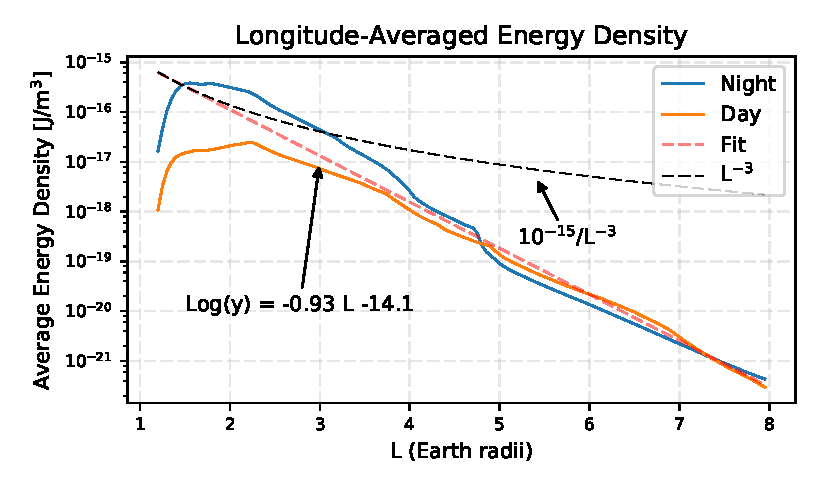
\includegraphics{figures/density_vs_L_with_fit.pdf}
\caption[Average energy density vs L, longitude-averaged]{Global, longitude-averaged energy density for day and night. The energy density is logarithmic with increasing L. The dashed black line shows an approximate 1/R$^3$ trend, in comparison with an isotropic radiator.}
\label{fig:energy_density_vs_L_trendline}
\end{center}
\end{figure}

\begin{figure}[h!]
\begin{center}
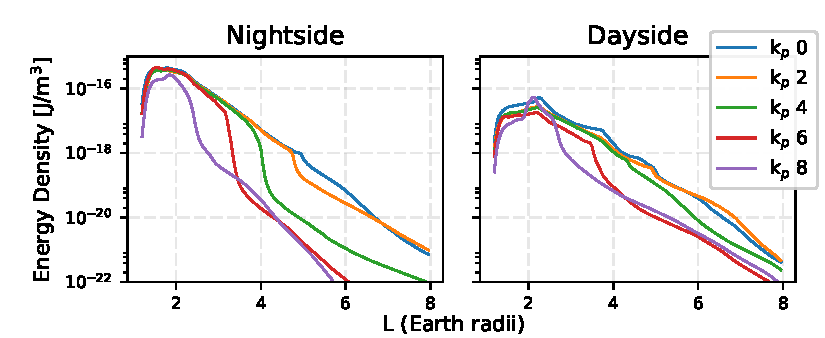
\includegraphics{figures/density_vs_L_multiple_kp.pdf}
\caption[Average energy density vs L for multiple K$_p$]{Average energy density for day and night, as in Figure \ref{fig:energy_density_vs_L_trendline}, broken out over multiple values of K$_p$. At higher K$_p$, the plasmapause effectively confines wave energy to the inner plasmasphere.}
\label{fig:energy_density_vs_L_multiple_kp}
\end{center}
\end{figure}

\paragraph{Frequency dependence}
We can examine the frequency spectrum resulting from lightning as a function of L-shell, as shown in Figure \ref{fig:energy_density_vs_L_vs_freq}. Generally, as seen in Figure \ref{fig:raytracing_example}, lower-frequency rays propagate further out into the magnetosphere, while higher-frequency rays are strongly-deflected and impact the Earth before a single magnetospheric reflection. This trend results in rays ``settling'' onto specific fieldlines, dependent on frequency.

The relationship between peak frequency and L-shell is well-defined by a logarithmic fit:
\begin{equation}
\label{eqn:frequency_fit}
\mathrm{log}_{10}(f_{peak}) = 4.56 - 0.48 L
\end{equation}

An additional feature of note in Figure \ref{fig:energy_density_vs_L_vs_freq} is the broad range of frequencies present at L $\sim$ 2.3, the location of which strongly supports the hypothesis of lightning as a key mechanism for slot region depletion. 
\begin{figure}[hb]
\begin{center}
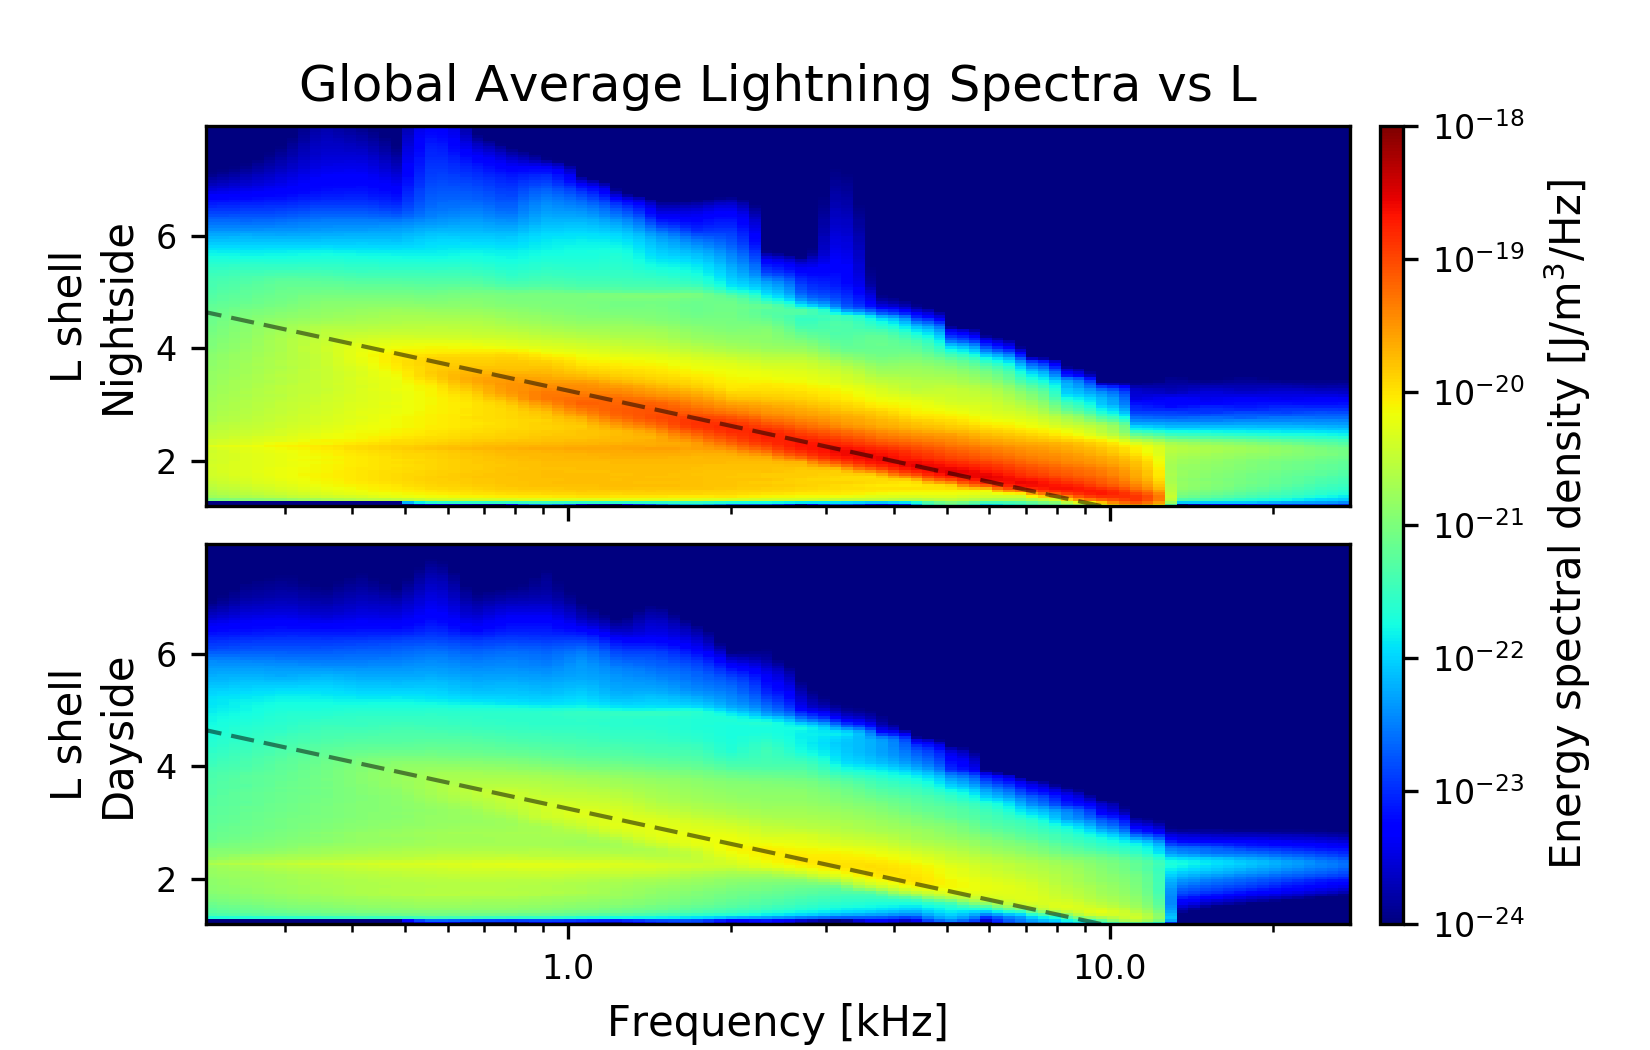
\includegraphics{figures/lightning_spectra_vs_L_logscale.png}
\caption[Average energy density vs L and frequency]{Average energy density as a function of L-shell and wave frequency. Dashed lines show a log-linear fit to the peak frequency as a function of L-shell in equation \eqref{eqn:frequency_fit}.}
\label{fig:energy_density_vs_L_vs_freq}
\end{center}
\end{figure}











